\documentclass[xcolor=svgnames,dvipsnames,table, hyperref=pdftex, mathserif, presentation]{beamer}
\usepackage{amsmath,amssymb,amsfonts,amsthm}
\usepackage{ctex}
\usepackage{graphics}
\usepackage{graphicx}
\usepackage{xcolor}
\usepackage{wasysym}
\usepackage{bbm}
\usepackage{url}
\usepackage{beamerleanprogress}
\usepackage{tikz-dependency}
\usepackage{tikz-qtree}
\usepackage{multirow}

\newcommand{\tabincell}[2]{\begin{tabular}{@{}#1@{}}#2\end{tabular}}%放在导言区
\usetheme{CambridgeUS}
%\usetheme{Pittsburgh}
\usecolortheme{orchid} % seahorse  orchid rose
\setbeamertemplate{blocks}[rounded][shadow=true]
\AtBeginSection[]{%
  \begin{frame}<beamer>
    \frametitle{Outline}
      \tableofcontents[current] 
    \end{frame}
  \addtocounter{framenumber}{-1}% If you don't want them to affect the slide number
}
\AtBeginSubsection[]
{
  \begin{frame}
  \frametitle{Outline}
    \tableofcontents[currentsection,currentsubsection]
  %\tableofcontents[sectionstyle=show/hide,subsectionstyle=hide/show/hide]
  \end{frame}
  \addtocounter{framenumber}{-1}% If you don't want them to affect the slide number
}
\newcommand{\setof}[1]{\ensuremath{\left \{ #1 \right \}}}
\newcommand{\tuple}[1]{\ensuremath{\left \langle #1 \right \rangle }}
\newcommand{\red}[1]{\textcolor{red}{#1}}
\newcommand{\brown}[1]{\textcolor{brown}{#1}}
\newcommand{\green}[1]{\textcolor{green}{#1}}
\newcommand{\blue}[1]{\textcolor{blue}{#1}}
\newcommand{\cyan}[1]{\textcolor{cyan}{#1}}

%gets rid of navigation symbols
\setbeamertemplate{navigation symbols}{}

\begin{document}

\title[2014秋总结]{2014秋季学期总结}

\institute[icst@pku]{
  
}
\author[Zhe Han]{\\ 韩喆 \\  iampkuhz@gmail.com
}

\frame[t,plain]{ \titlepage } % [t,plain]

\frame{
  \frametitle{ Outline  }
  
   \begin{itemize}

  \item 研究生课程

  \item 实验室工作
    \begin{itemize}
    \item 新华社
    \item 基于中文维基百科的知识库
    \end{itemize}
   
   \item 总结和展望
   
  \end{itemize}
}

\frame{
    \centering
    \begin{Large}
     研究生课程
    \end{Large}


  \begin{block}{研究生课程(15学分)}
  \begin{itemize}
   \item \begin{footnotesize}
          必修:算法分析和复杂性理论(3)、自然辩证法概论(1)、国际英语视听说(2)
         \end{footnotesize}
   \item \begin{footnotesize}
          选修:语义计算与知识检索(3)、计算语言学(3)、模式识别(3)
         \end{footnotesize}
  \end{itemize}
  \end{block}
}


\frame{
  \frametitle{ Courses  }
  
   \begin{itemize}


  \item 计算语言学
    \begin{itemize}
    \item 介绍基础的自然语言处理模型和方法,适合入门,内容不是很新,有相关基础的可能在课堂上学不到太多新的知识
    \item 大作业:复述检测(77.27\%准确率,应该是班里最好的)
	\begin{itemize}
	 \item 方法:各种特征暴力叠加+分类器投票;state-of-art:77.6\%
	\end{itemize}

    \end{itemize}
   
  \item 语义计算与知识检索
    \begin{itemize}
    \item 信息检索有关的知识,可以在实验中提供不少思路和小经验
    \item 大作业:中文问答(模型简单,效果不好...);小作业:豆瓣电影评分
    \end{itemize}
   
  \item 模式识别
    \begin{itemize}
    \item 智能系任选,比较偏理论推导,没有基础,听得比较吃力。
    \item 了解了一些神经网络在自然语言中的应用
    \end{itemize}
   
  \end{itemize}
}


\frame{
  \frametitle{ Courses  }
  
   \begin{itemize}

  \item 个人总结
    \begin{itemize}
    \item 各门课难度不一
	\begin{itemize}
	 \item 算法分析、模式识别难度较大,需要花一些时间
	 \item 全校必修、计算语言学很水,求过的话不用花什么时间...
	\end{itemize}

    \item 作业模式有了不少转变
	\begin{itemize}
	 \item 作业:查论文->实现论文
	\end{itemize}


    \end{itemize}
  \end{itemize}
}


\frame{
    \centering
    \begin{Large}
     实验室工作
    \end{Large}


  \begin{block}{` }
  \begin{itemize}
   \item \begin{footnotesize}
          新华社:新闻展示网站、新闻标注网站
         \end{footnotesize}
   \item \begin{footnotesize}
          基于中文维基百科的知识库
         \end{footnotesize}
   \item \begin{footnotesize}
          其余工作
         \end{footnotesize}
  \end{itemize}
  \end{block}
}


\frame{
  \frametitle{ Lab  }
  
   \begin{itemize}

  \item 新华社
    \begin{itemize}
    \item 新闻展示网站
	\begin{itemize}
	 \item 新闻中的实体链接到中文维基百科知识库
	 \item 展示新闻中实体之间的关系
	\end{itemize}

    \item 新闻标注网站
	\begin{itemize}
	  \item \begin{footnotesize}
	         和曾颖一起负责。将组里抓取的各个网站的新闻汇集起来,交由志愿者进行ccnc类别标注
	        \end{footnotesize}
	  \item 我:生成新闻数据,半自动检测志愿者标注效果
	  \item zy:搭建新闻标注网站。
	  \item 进度:进行中。已标注7000篇,7名志愿者
	\end{itemize}


    \end{itemize}
  \end{itemize}
}


\frame{
  \frametitle{ Lab  }
  
   \begin{itemize}

  \item 基于中文维基百科的知识库
    \begin{itemize}
    \item 学期前进展(毕设工作)
	\begin{itemize}
	 \item 1100多万三元组(830多万高质量三元组)
	      \begin{block}{}
		  \begin{center}
		   低质量三元组:【\red{中国}:\green{职位1}:\blue{国家主席}】  【\red{中国}:\green{人物1}:\blue{习近平}】  
		  \end{center}
	      \end{block}
	 
	\end{itemize}

    \item 问题/不足
	\begin{itemize}
	  \item 和百度百科的实体链接基于名称(字符串),且百度百科三元组较少
	  \item 未和其他中文知识库链接(但是已和英文维基百科知识库链接)
	  \item \textbf{谓词很多非中文(一半以上)}:\red{本学期工作}
	      \begin{block}{}
	       \centering
	       \begin{figure}
	        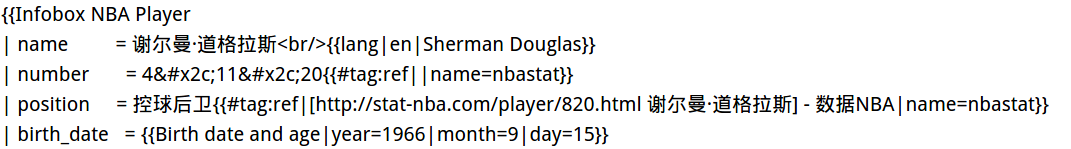
\includegraphics[width=0.9\textwidth]{wikitextEngPred.png}
	       \end{figure}
	      \end{block}

	\end{itemize}


    \end{itemize}
  \end{itemize}
}

\frame{
  \frametitle{ Lab  }
  
   \begin{itemize}

  \item 基于中文维基百科的知识库
    \begin{itemize}
    \item 本学期工作中心
	\begin{itemize}
	 \item 中文维基百科谓词标准化/归一化。
	 \begin{block}{}
	  \centering 建筑商、建筑单位、承建商、主承建商、建商、设计建设团队、建造所
	 \end{block}
	 \item 启发式规则筛掉错误三元组/谓词;抽取谓词的特征,设计分类器判断任意两个谓词是否描述相同实体
	  \item 目标:生成一个内部统一的谓词体系(schema),合并其他知识库

	\end{itemize}

    \item 本学期工作(已完成)
	\begin{itemize}
	 \item 完成了\red{基于中文维基百科网页的三元组抽取}
	 \item 650万高质量三元组,谓词符合直观
	 \item 谓词规模:2.6w -> 1.5w (筛除错误三元组)
	 \item \red{基于网页抽取的三元组}和\blue{基于wikitext抽取的三元组}对应(启发规则)
	 \item 已抽特征:对应的wikitext的内容、上级标题、单词特征...
	 \item 制作了一个版本给彭宇新老师组使用
	 
	\end{itemize}
    \end{itemize}
  \end{itemize}
}


\frame{
  \frametitle{ Lab  }
  
   \begin{itemize}

  \item 基于中文维基百科的知识库(进行中)
    \begin{itemize}
    \item 模仿新闻标注网站写了一个谓词的标注网页,手工标注,排除错误谓词(8k/15k)
    \item 基于一些启发式规则标注训练数据(谓词二元组)
    \item 抽取出谓词的相关特征,进行测试和改进
    \end{itemize}
    \begin{block}{}
     \begin{figure}
      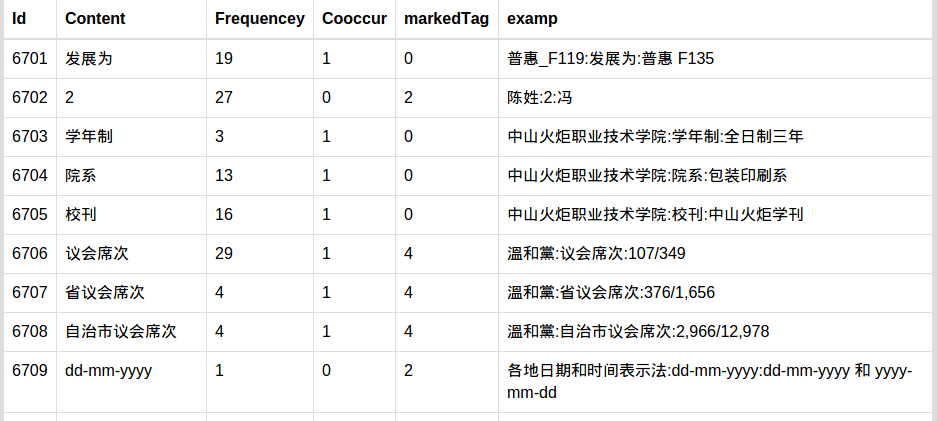
\includegraphics[width=0.6\textwidth]{editPredicateInfo.png}
     \end{figure}

    \end{block}

  \end{itemize}
}


\frame{
  \frametitle{ Lab  }
  
   \begin{itemize}

  \item 其余工作
    \begin{itemize}
    \item 中英文所有的维基百科网页、dump都已经抓下来了,大家可以使用
    \item 帮助许坤和张晟做了一点和英文维基百科有关的抓取任务。
    \item 参与冯老师小组的论文讨论班
    \end{itemize}

  \end{itemize}
}

\frame{
    \centering
    \begin{Large}
     总结和展望
    \end{Large}
    
  \begin{block}{` }
  \begin{center}
   latex,paper,计划/备忘录,托福...
  \end{center}

  \end{block}
}

\frame{
  \frametitle{ Summary  }
  
   \begin{itemize}

    \item 优点
	\begin{itemize}
	 \item 养成使用latex的习惯了:所有的报告和大部分作业
	 \item 看了一些论文:仔细看过20多篇论文
	    \begin{itemize}
	     \item 起因:写大作业、讨论班、找实验方法...
	     \item 速度提高:半天->2个小时
	    \end{itemize}
	\end{itemize}
    \item 失败
	\begin{itemize}
	 \item 每周两篇paper
	 \item 每天的备忘录、背托福单词等诸多问题
	\end{itemize}

    \item 缺点/不足
	\begin{itemize}
	 \item 做事缺少计划性
	    \begin{itemize}
	     \item 开学的时候谓词任务做了不少,快期中的时候就突然不想做了,直到前一周才做
	    \end{itemize}

	\end{itemize}

  \end{itemize}
}

\frame{
  \frametitle{ Summary  }
  
   \begin{itemize}

    \item 下学期展望
	\begin{itemize}
	 \item 背单词,考托福
	 \item 结束研究生课程内容
	 \item 完成中文知识库谓词归一,链接其余知识库
	\end{itemize}
    \item (同之前的失败项)
	\begin{itemize}
	 \item 每周两篇paper
	 \item 每天的备忘录、背托福单词等诸多问题
	\end{itemize}

  \end{itemize}
}


\frame{
    \centering
    \begin{Large}
     谢谢大家!
    \end{Large}
}
\end{document}
